%%%--- Template for master thesis at SfS
%%%--- Modified template with more comments and examples -- SG, 11/06/09
%%%------
\documentclass[11pt,a4paper,twoside,openright]{report}
%%not needed \usepackage{E}
\usepackage[utf8]{inputenc}
\usepackage[english]{style/ETHDAsfs}%--> ETHDASA + fancyheadings + ... "umlaute"
%  + sfs-hyper -> hyperref

\usepackage{pdfpages}%%to include the confirmation of originality (plagiarism
\usepackage{amsbsy}%% for \boldsymbol and \pmb{.}
\usepackage{amssymb}%% calls  amsfonts...
\usepackage{booktabs} % For \toprule etc. in tables
\usepackage[table]{xcolor} 
%or \usepackage{german8}%-- =  german  +  isolatin1
\usepackage{graphicx}%-- f?r PostScript-Grafiken (besser als  psfig!)
%\usepackage[draft]{graphicx} % grafics shown as boxes --> faster compilation
%
\usepackage[longnamesfirst]{natbib}%was {sfsbib}%- F?r  Literatur-Referenzen
%           ^^^^^^^^^^^^^^ 1) "Hampel, Ronchetti, ..,"  2) "Hampel et al"
% Engineers (and other funny people) want to see [1], [2]
% ---> use 'numbers' : \usepackage[longnamesfirst,number]{natbib}
%
%
\usepackage{style/texab}%- 'tex Abk?rzungen' /u/sfs/tex/tex/latex/texab.sty
        %%- z.B.  \R, \Z, \Q, \Nat f?r reelle, ganze, rationale, nat?rl. Zahlen;
        %%-       \N   (Normalvert.)  \W == Wahrscheinlichkeit .....
        %%-  \med, \var, \Cov, \....
        %%-  \abs{x} == |x|   und   \norm{y} ==  || y ||   (aber anst?ndig)
%% NOTE: texab contains many useful definitions and "shortcuts". It is
%% worth to open the file and have a look at them. HOWEVER, some
%% definitions can lead to conflicts with other packages. You
%% might for example want to comment out the line defininf \IF as an
%% operator when working with the algorithmic package, or to comment out
%% the line defining a command \Cite with working with the Biblatex package
\usepackage{amsmath}
%\usepackage{mathrsfs}% Raph Smith's Formal Script font --> provides \mathscr
\usepackage{enumerate}% Fuer selbstdefinierte Nummerierungen
%--------
\usepackage{relsize}%-> \smaller (etc) used here
\usepackage{color} %% to allow cloring in code listings
\usepackage{listings}% Fuer R-code, C-code, ....  and settings for these:
\definecolor{Mygrey}{gray}{0.75}% for linenumbers only!
\definecolor{Cgrey}{gray}{0.4}% for comments
\lstloadlanguages{R}
\lstset{ %% Hilfe unter z.B. http://en.wikibooks.org/wiki/LaTeX/Packages/Listings
language=R,
basicstyle=\ttfamily\scriptsize,%%- \small > \footnotesize > \scriptsize > \tiny
%commentstyle=\ttfamily\color{Cgrey},
commentstyle=\itshape\color{Cgrey},
numbers=left,
numberstyle=\ttfamily\color{Mygrey}\tiny,
stepnumber=1,
numbersep=5pt,
backgroundcolor=\color{white},
showspaces=false,
showstringspaces=false,
showtabs=false,
frame=single,
tabsize=2,
captionpos=b,
breaklines=true,
%breakatwhitespace=false,
keywordstyle={},
morekeywords={},
xleftmargin=4ex,
literate={<-}{{$$\leftarrow$$}}1 {~}{{$$\sim$$}}1}
\lstset{escapeinside={(*}{*)}} % for (*\ref{ }*) inside lstlistings (Scode)
%%----------------------------------------------------------------------------

%%------- Theoreme ---
\newtheorem{definition}{Definition}[subsection]
\newtheorem{lemma}[definition]{Lemma}
\newtheorem{theorem}[definition]{Theorem}
\newtheorem{Coro}[definition]{Corollary}
\theoremstyle{definition}
\newtheorem{example}[definition]{Example}
\newtheorem*{note}{Note}
\newtheorem*{remark}{Remark}

\DeclareMathOperator*{\plim}{plim}
% \def\MR#1{\href{http://www.ams.org/mathscinet-getitem?mr=#1}{MR#1}}

% \newcommand{\Lecture}[3]{\marginpar{#3.#2.#1}}
% \newcommand{\Fu}{\mathcal{F}}
\newcommand{\aatop}[2]{\genfrac{}{}{0pt}{}{#1}{#2}}

%\renewcommand{\theequation}{\arabic{equation}}
\numberwithin{equation}{subsection}

%%%%%%%%%%%%%%%%%%%%%%%%%%%%%%%%%%%%%%%%%%%%%%%%%
%%% Path for your figures                      %%%
%%%%%%%%%%%%%%%%%%%%%%%%%%%%%%%%%%%%%%%%%%%%%%%%%
% Set the paths where all figures are taken from:
\graphicspath{{images/}}

%%%%%%%%%%%%%%%%%%%%%%%%%%%%%%%%%%%%%%%%%%%%%%%%%
%%% Define your own commands here             %%%
%%%%%%%%%%%%%%%%%%%%%%%%%%%%%%%%%%%%%%%%%%%%%%%%%
\newcommand{\Bruch}[2]{{}^{#1}\!\!/\!_{#2}}
\renewcommand{\labelenumi}{\roman{enumi}.)}
\providecommand{\tightlist}{%
  \setlength{\itemsep}{0pt}\setlength{\parskip}{0pt}}

$header-includes$
$if(highlighting-macros)$
$highlighting-macros$
$endif$

\begin{document}
\bibliographystyle{style/chicago}% ---> Hampel,F., E.Ronchetti,... W.Stahel(1986) ...
 %was \bibliographystyle{sfsbib}\citationstyle{dcu} %OR DEFAULT : \citationstyle{agsm}

\pagenumbering{roman}%- roman numbering for first few pages

%%%%%%%%%%%%%%%%%%%%%%%%%%%%%%%%%%%%%%%%%%%%%%%%%
%%% Title page                                %%%
%%%%%%%%%%%%%%%%%%%%%%%%%%%%%%%%%%%%%%%%%%%%%%%%%
\period{$date$}
\dasatype{Master Thesis}
\students{$author$}
$if(coadviser)$
\alternatereaderprefix{Co-Adviser:}
\alternatereader{$coadviser$}
\mainreaderprefix{Adviser:}
\mainreader{$adviser$}
$else$
\alternatereaderprefix{Adviser:}
\alternatereader{$adviser$}
\mainreaderprefix{}
\mainreader{}
$endif$


\submissiondate{$submission_date$}
\title{$title$}

\maketitle%- Titelseite wird abgeschlossen
\cleardoublepage
 %%~~~~~~~~~~~~~~~~~~~~~~~~~~~~~~~~~~~~~~~~

%%%%%%%%%%%%%%%%%%%%%%%%%%%%%%%%%%%%%%%%%%%%%%%%%
%%% Insert here acknowledgements and abstract %%%
%%%%%%%%%%%%%%%%%%%%%%%%%%%%%%%%%%%%%%%%%%%%%%%%%
%% Dedication (optional)
\markright{}
\vspace*{\stretch{1}}
\begin{center}
    To some special person
\end{center}
\vspace*{\stretch{2}}

% Preface (optional)
\newpage
\markboth{Preface}{Preface}
\chapter*{Preface}

I would like to extend my gratitude to all the people that supported me throughout the this project. To Matthias, that from the start of my interest in this field, inspired and challenged me to create something new. You taught me many lessons that will stay with me and I value enormously the interesting conversations that stimulated a lot of excitment and creativity. To Maybritt, thank you for your support, insights, supervision and the many conversations that inspired solutions. Your encouragements from the start to the end were incredibily valuable. To Belinda, your help was essential in fortifying my physics competences and I appreciated the time you spend supporting my work. To Heini, thank you for the supervision and feedback that was instrumental in shaping a meaningul and impactful project. You all showed interest in my work and I am very grateful to have had such a competent, enthusiastic and friendly team.

This thesis has been a unique opportunity to place myself at the head of a scientific project, and it was foremost a humbling experience, as the challenges of interdisplinary research have taught me. Throughout all the ups and down, I would like to thank my friends for the moments of laughter, for being great rubber ducks, and for all the good times. I will miss you all a lot and am eager to follow all your future adventures. Grazie mamma per essere stata sempre raggiungibile, per le poesie ispirante e le foto del grigio che mi fanno sorridere molto. Merci papa pour ces parties de ping-pong qui me sont si importantes et les bons verres de vins. To Matt and Luca, always wonderful to have you around: I cherish all the moments we have together. To my Manu, thank you for everything. Your calls and visits brought me joy and comfort, our time together is so dear to me and you are always an inspiration. I am so glad to have you by my side. 


%%% Local Variables: 
%%% mode: latex
%%% TeX-master: "MasterThesisSfS"
%%% End: 


% Abstract should not be longer than one page.
\newpage
\markboth{Abstract}{Abstract}
\chapter*{Abstract}

Heat-related extremes are important meteorological phenomena that can have strong consequences on human health and the environment. Climate change is expected to exacerbate these impacts through an increase in the frequency of hot extreme occurrence and intensity. Although there exists abundant literature on the typical physical functioning of these events and their association to the variability of the climate system on different temporal scales, there lacks a global assessment of the influence of major physical processes - heat advection, adiabatic compression and diabatic heating - on the yearly variation of hot extreme magnitudes. To remediate this knowledge gap, we first propose a data-driven, systematic analysis of second-moment characteristics of yearly maxima near-surface hot extreme events and contributing heat-generating processes. Second, we apply deep-learning methods to model hot extreme Lagrangian trajectories to gain insights into important dynamical features. No physical process is globally found to dominate variability in these events and significant variance contributions exist from at least two processes, suggesting that mean-state understanding of hot extreme development may not not be sufficient to explain large year-to-year differences in their magnitudes. Furthermore, this analysis reaffirms the presence of strong dependencies between the three physical mechanisms leading to a characterization of their variability by only one or two degrees of freedom in most of the world. Finally, the approach for the analysis of parcel trajectories was limited due to generally poor predictive performance, but showed that the patterns in advective, adiabatic and diabatic temperature anomaly generation follow patterns that may be predicted from their history, encouraging for future work. In addition, over oceans and many land regions we observe that adiabatic heating is minimal during the final 24h, suggesting that hot extreme primarily descend to the surface earlier than a day before, thus leading to contributions from advective and diabatic processes more likely.

%%% Local Variables: 
%%% mode: latex
%%% TeX-master: "MasterThesisSfS"
%%% End: 



%%%%%%%%%%%%%%%%%%%%%%%%%%%%%%%%%%%%%%%%%%%%%%%%%
%%% Table of contents and list of figures and %%%
%%% tables (no need to change this usually)   %%%
%%%%%%%%%%%%%%%%%%%%%%%%%%%%%%%%%%%%%%%%%%%%%%%%%
\newpage
\tableofcontents
\newpage
\listoffigures
\newpage
\listoftables

%% Notations and glossary (optional)
\cleardoublepage
\phantomsection
\addcontentsline{toc}{chapter}{\protect\numberline{}{Notation}}
\markboth{Notation}{Notation}
\chapter*{Notation}
\label{c:Notation}

Explain your symbols and abbreviations.

%%% Local Variables: 
%%% mode: latex
%%% TeX-master: "MasterThesisSfS"
%%% End: 


\cleardoublepage
\pagenumbering{arabic}%--- switch back to standard numbering


%%%%%%%%%%%%%%%%%%%%%%%%%%%%%%%%%%%%%%%%%%%%%%%%%
%%% Your text... Either write here directly,  %%%
%%% or even better: write in separate files   %%%
%%% that you just have to include here.       %%%
%%%%%%%%%%%%%%%%%%%%%%%%%%%%%%%%%%%%%%%%%%%%%%%%%
$body$
%%%%%%%%%%%%%%%%%%%%%%%%%%%%%%%%%%%%%%%%%%%%%%%%%
%%% Bibliography                              %%%
%%%%%%%%%%%%%%%%%%%%%%%%%%%%%%%%%%%%%%%%%%%%%%%%%
\addtocontents{toc}{\vspace{.5\baselineskip}}
\cleardoublepage
\phantomsection
\addcontentsline{toc}{chapter}{\protect\numberline{}{Bibliography}}
\bibliography{bib/bib}

%% All books from our library (SfS) are already in a BiBTeX file
%% (Assbib). You can use Assbib combined with your personal BiBTeX file:
%% \bibliography{Myreferences,Assbib}. Of course, this will only work on
%% the computers at SfS, unless you copy the Assbib file
%%  --> /u/sfs/bib/Assbib.bib

%%%%%%%%%%%%%%%%%%%%%%%%%%%%%%%%%%%%%%%%%%%%%%%%%
%%% Appendices (if needed)                    %%%
%%%%%%%%%%%%%%%%%%%%%%%%%%%%%%%%%%%%%%%%%%%%%%%%%
\addtocontents{toc}{\vspace{.5\baselineskip}}
\appendix
\chapter{Supplementary material on timeseries data}

\section{Further examples of trajectory data}

Find below the trajectory timeseries visualisation plots - as figure 4.2 - for the locations in figure 4.1. Each figure contains plots (a-d) of TX1day T’ decompositions for years 1980 to 2020. The x-axis is logarithmic to better represent the recent
 history. The trajectory yielding the largest final T’ among all years is colored red, the
 time-mean of all trajectories in black and the inter-quantile range is highlighted in light
 blue. It also contains the average auto-correlation (e) and cross-correlation with T’ (f) over all events
 for each contributor. The auto- and cross-correlation are computed for timeseries starting
 at genesis (ignoring padding) and timeseries that are smaller than 32 timesteps are not
 included in the averages for lags larger than their length.

\begin{figure}[h]
\caption{Location 28.5N 77E, in the vicinity of New Delhi, India.}
\centering
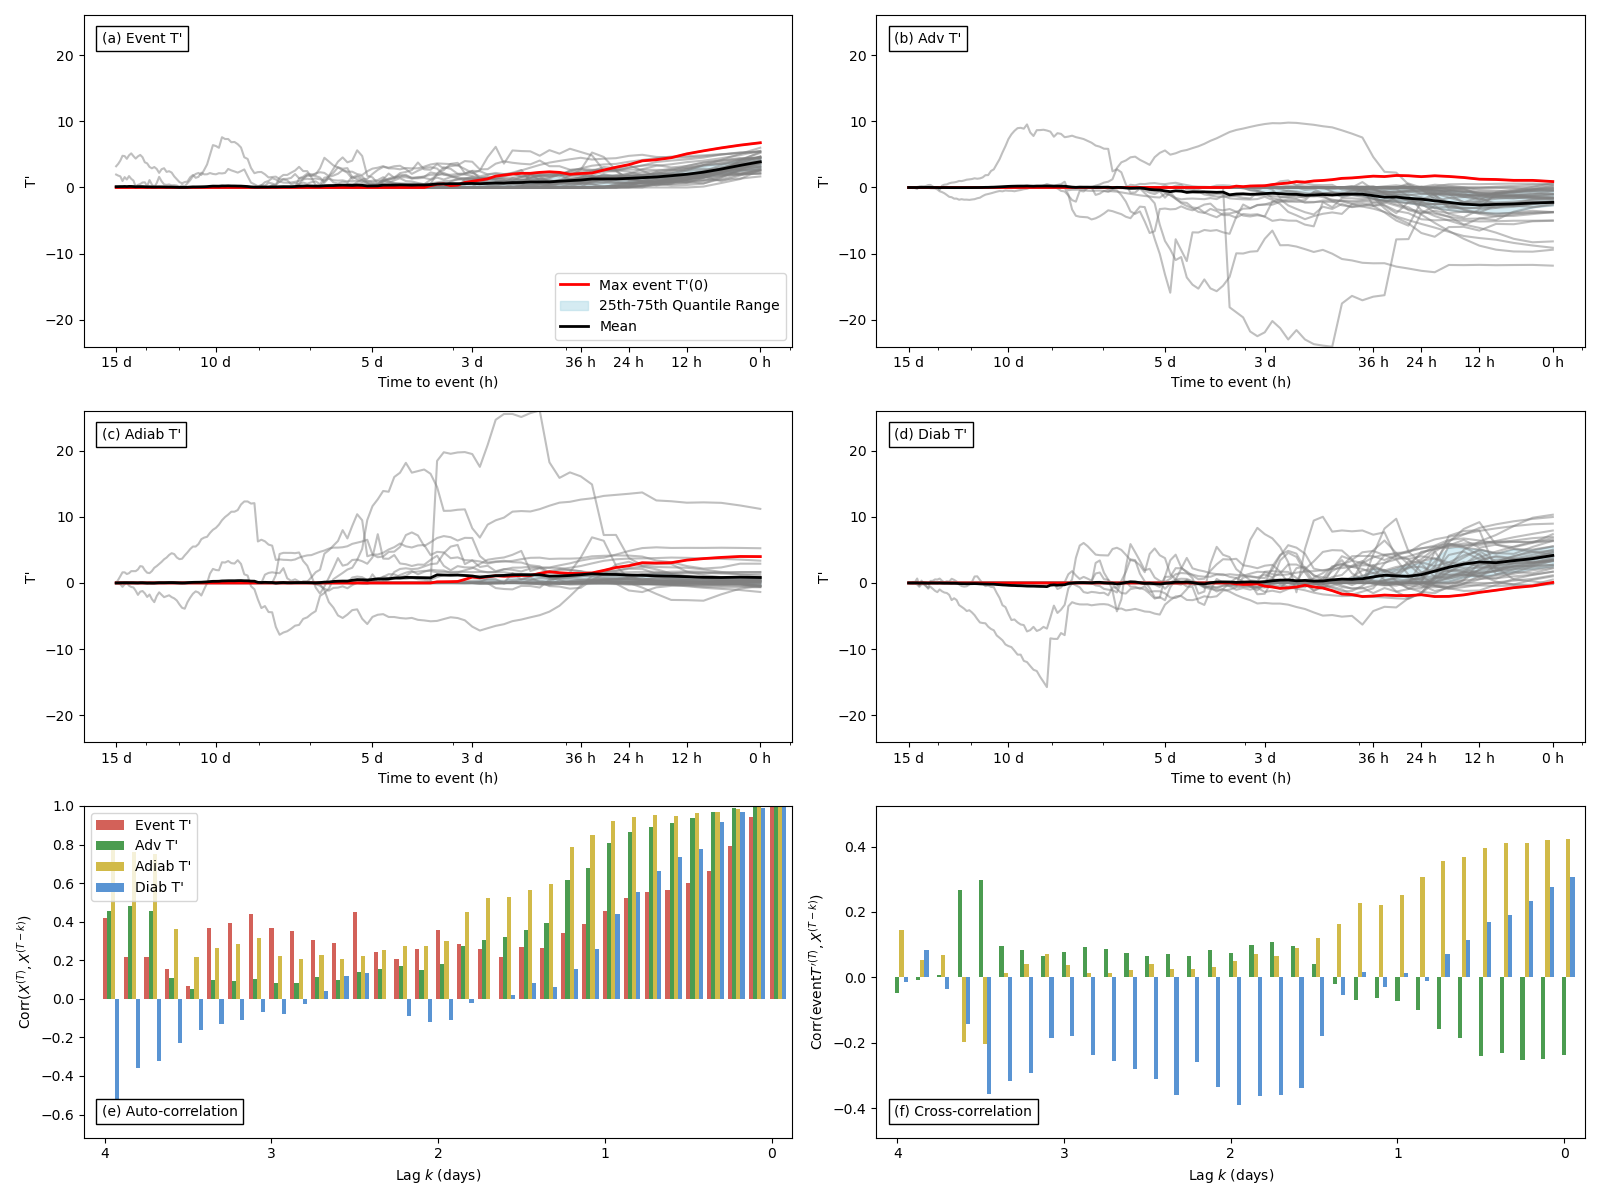
\includegraphics[width=0.9\textwidth]{images/sup1.png}
\end{figure}

\begin{figure}[h]
\caption{Location 45N 30W, in the middle of the Atlantic ocean.}
\centering
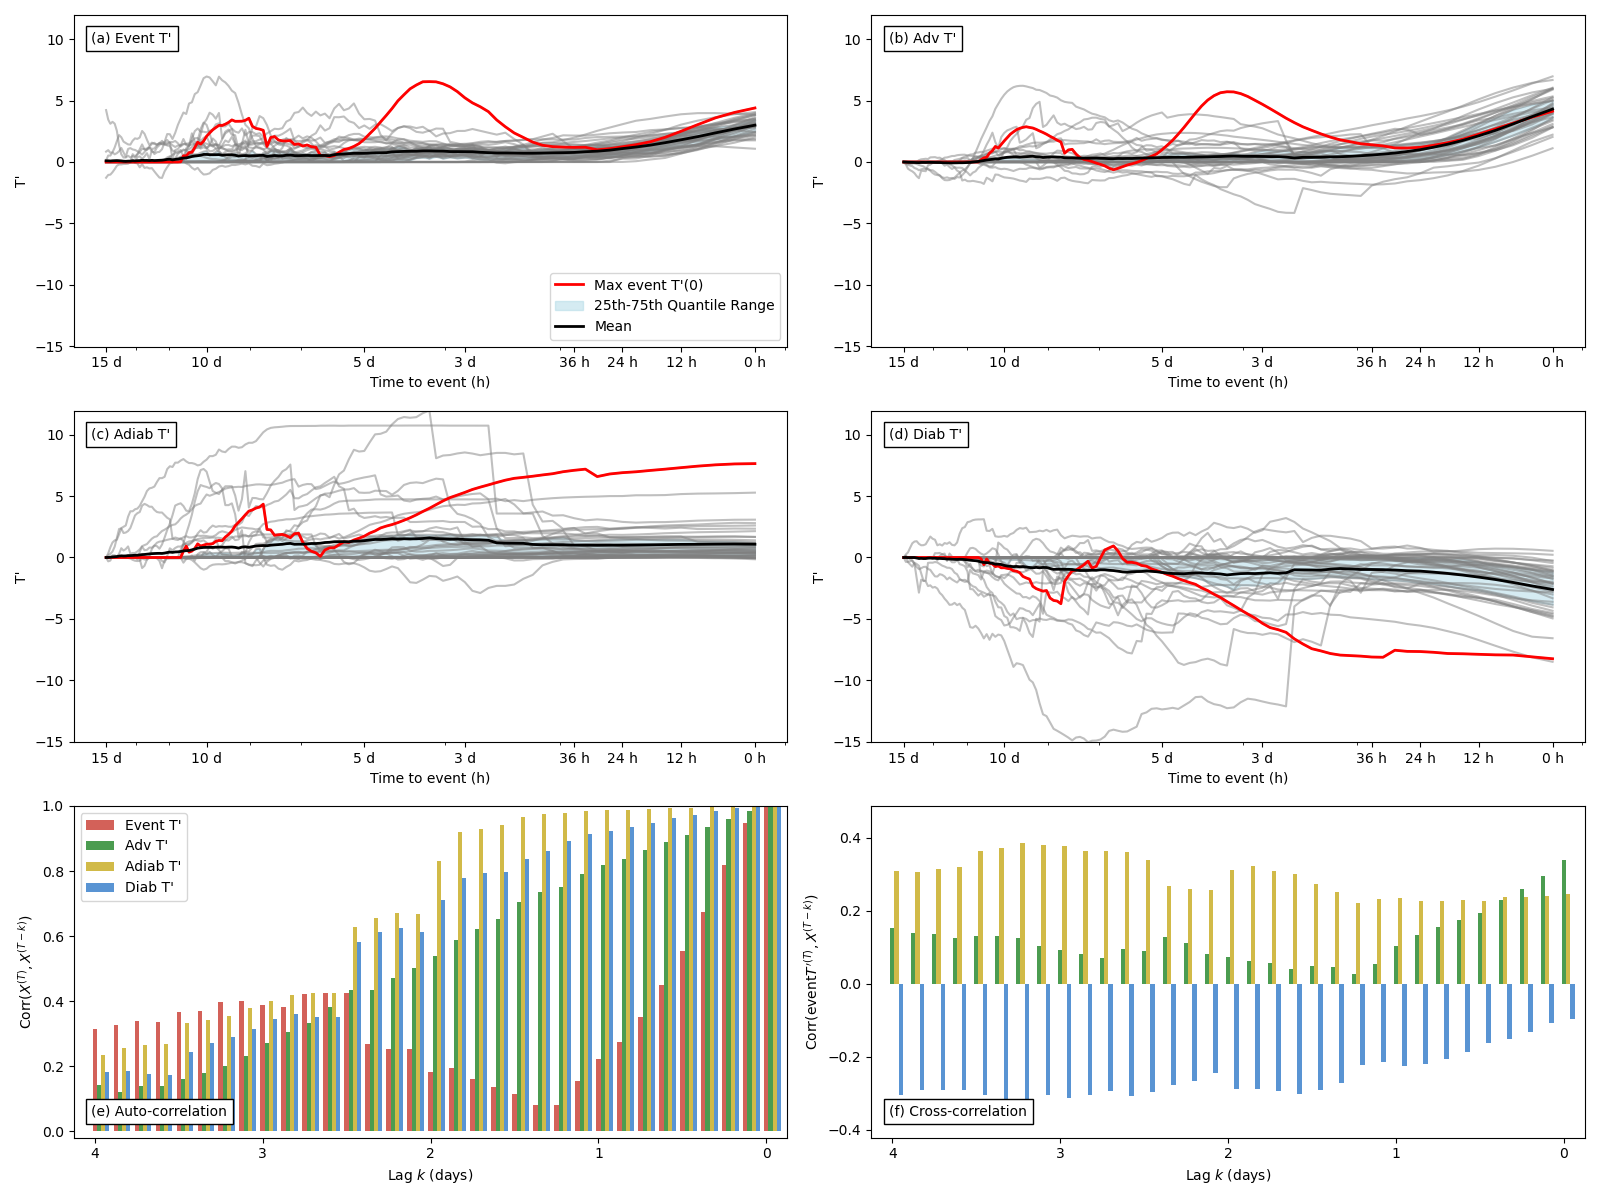
\includegraphics[width=0.9\textwidth]{images/sup2.png}
\end{figure}

\begin{figure}[h]
\caption{Location 32S 116E, in the vicinity of Perth, Australia.}
\centering
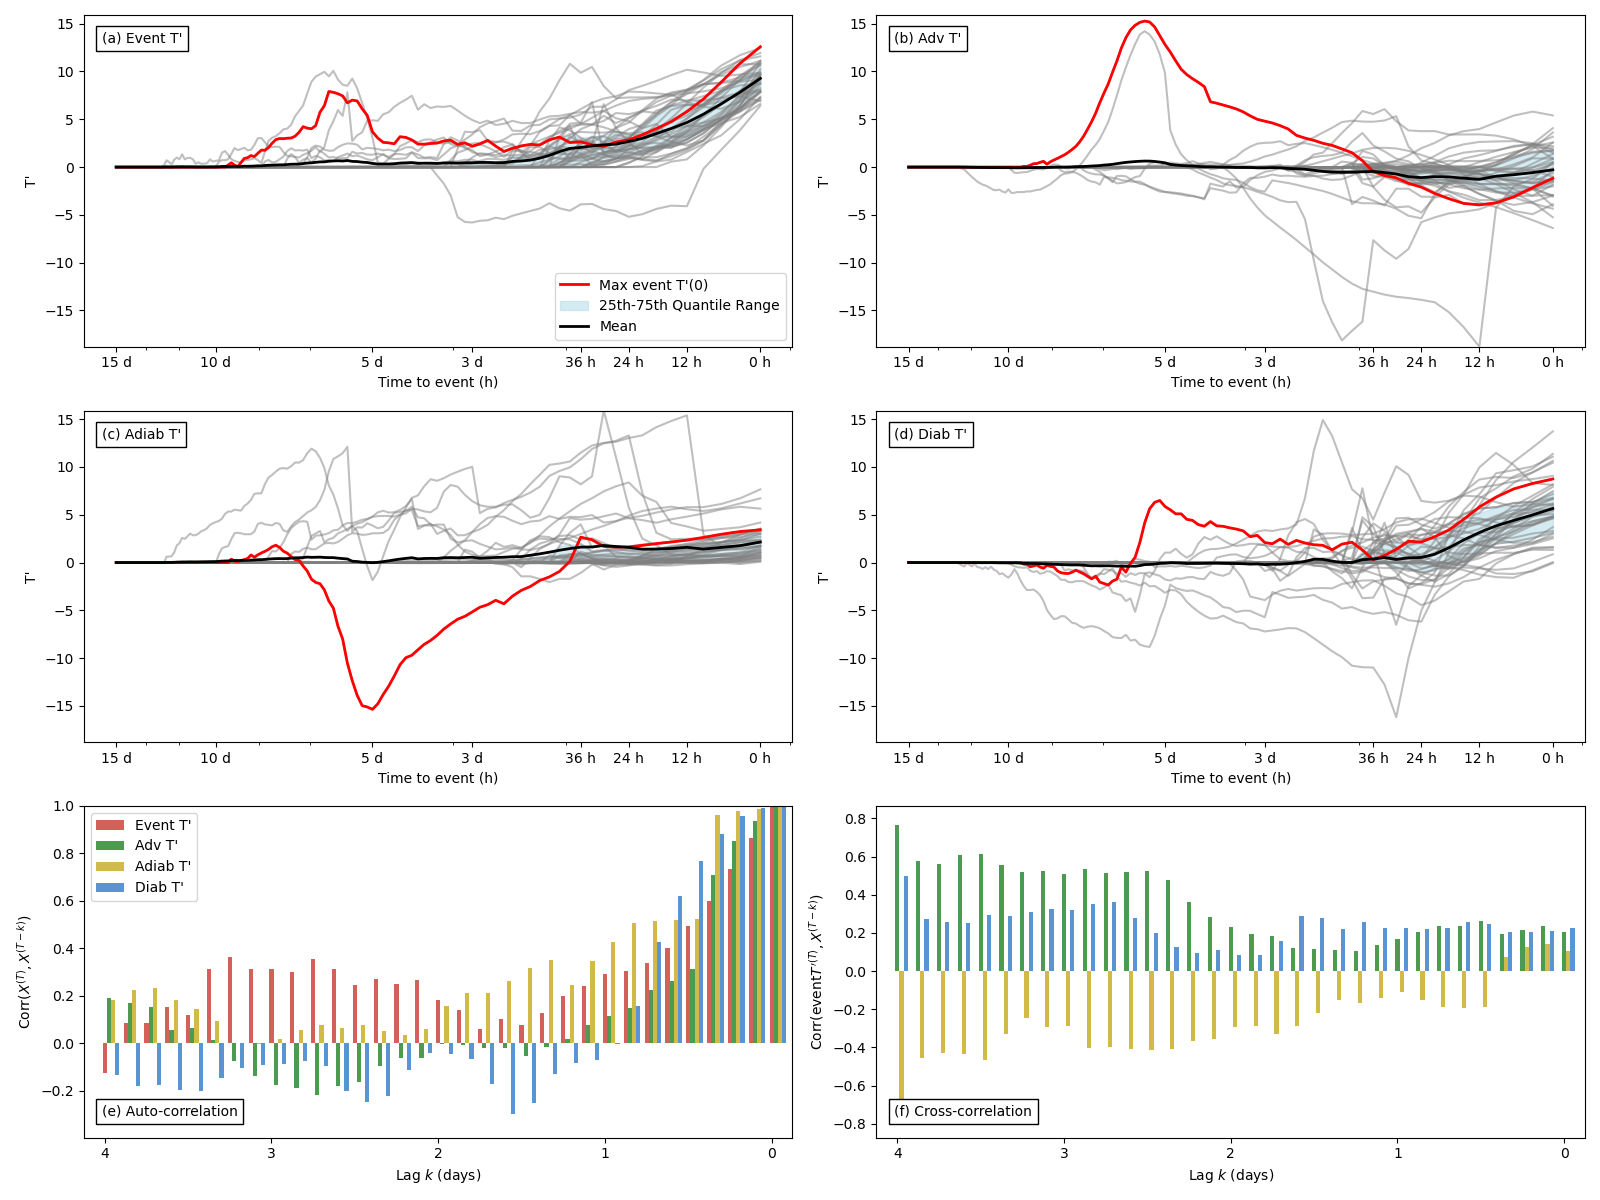
\includegraphics[width=0.9\textwidth]{images/sup3.png}
\end{figure}

\section{Differenced timeseries data}

%%% Local Variables: 
%%% mode: latex
%%% TeX-master: "MasterThesisSfS"
%%% End: 

\chapter{Yet another appendix....}

\section{Description}
\begin{description}
\item[Something] details.
\item[Something else] other definition.
\end{description}

\section{Tables}
Refer to Table~\ref{tab:example} to see a left justified table with caption
on top.

\begin{table}[ht]
\centering
\caption[Test results]{\label{tab:example}Results.}
\begin{tabular}{ll}
\hline
\textbf{Student} & \textbf{Grade}\\
\hline
Marie  & $6$\\
Alain  & $5.5$\\
Josette  & $4.5$\\
Pierre  & $5$\\
\hline
\end{tabular}
\end{table}

%%% Local Variables: 
%%% mode: latex
%%% TeX-master: "MasterThesisSfS"
%%% End: 



%% Epilogue (optional)
\addtocontents{toc}{\vspace{.5\baselineskip}}
\cleardoublepage
\phantomsection
\addcontentsline{toc}{chapter}{\protect\numberline{}{Epilogue}}
\markboth{Epilogue}{Epilogue}
\chapter*{Epilogue}
\label{s:Epilogue}

A few final words.



%%% Local Variables: 
%%% mode: latex
%%% TeX-master: "MasterThesisSfS"
%%% End: 



%%%%%%%%%%%%%%%%%%%%%%%%%%%%%%%%%%%%%%%%%%%%%%%%%%
%%% Declaration of originality (Do not remove!)%%%
%%%%%%%%%%%%%%%%%%%%%%%%%%%%%%%%%%%%%%%%%%%%%%%%%%
%% Instructions:
%% -------------
%% fill in the empty document confirmation-originality.pdf electronically
%% print it out and sign it
%% scan it in again and save the scan in this directory with name
%% confirmation-originality-scan.pdf
%%
%% General info on plagiarism:
%% https://www.ethz.ch/students/en/studies/performance-assessments/plagiarism.html
\cleardoublepage
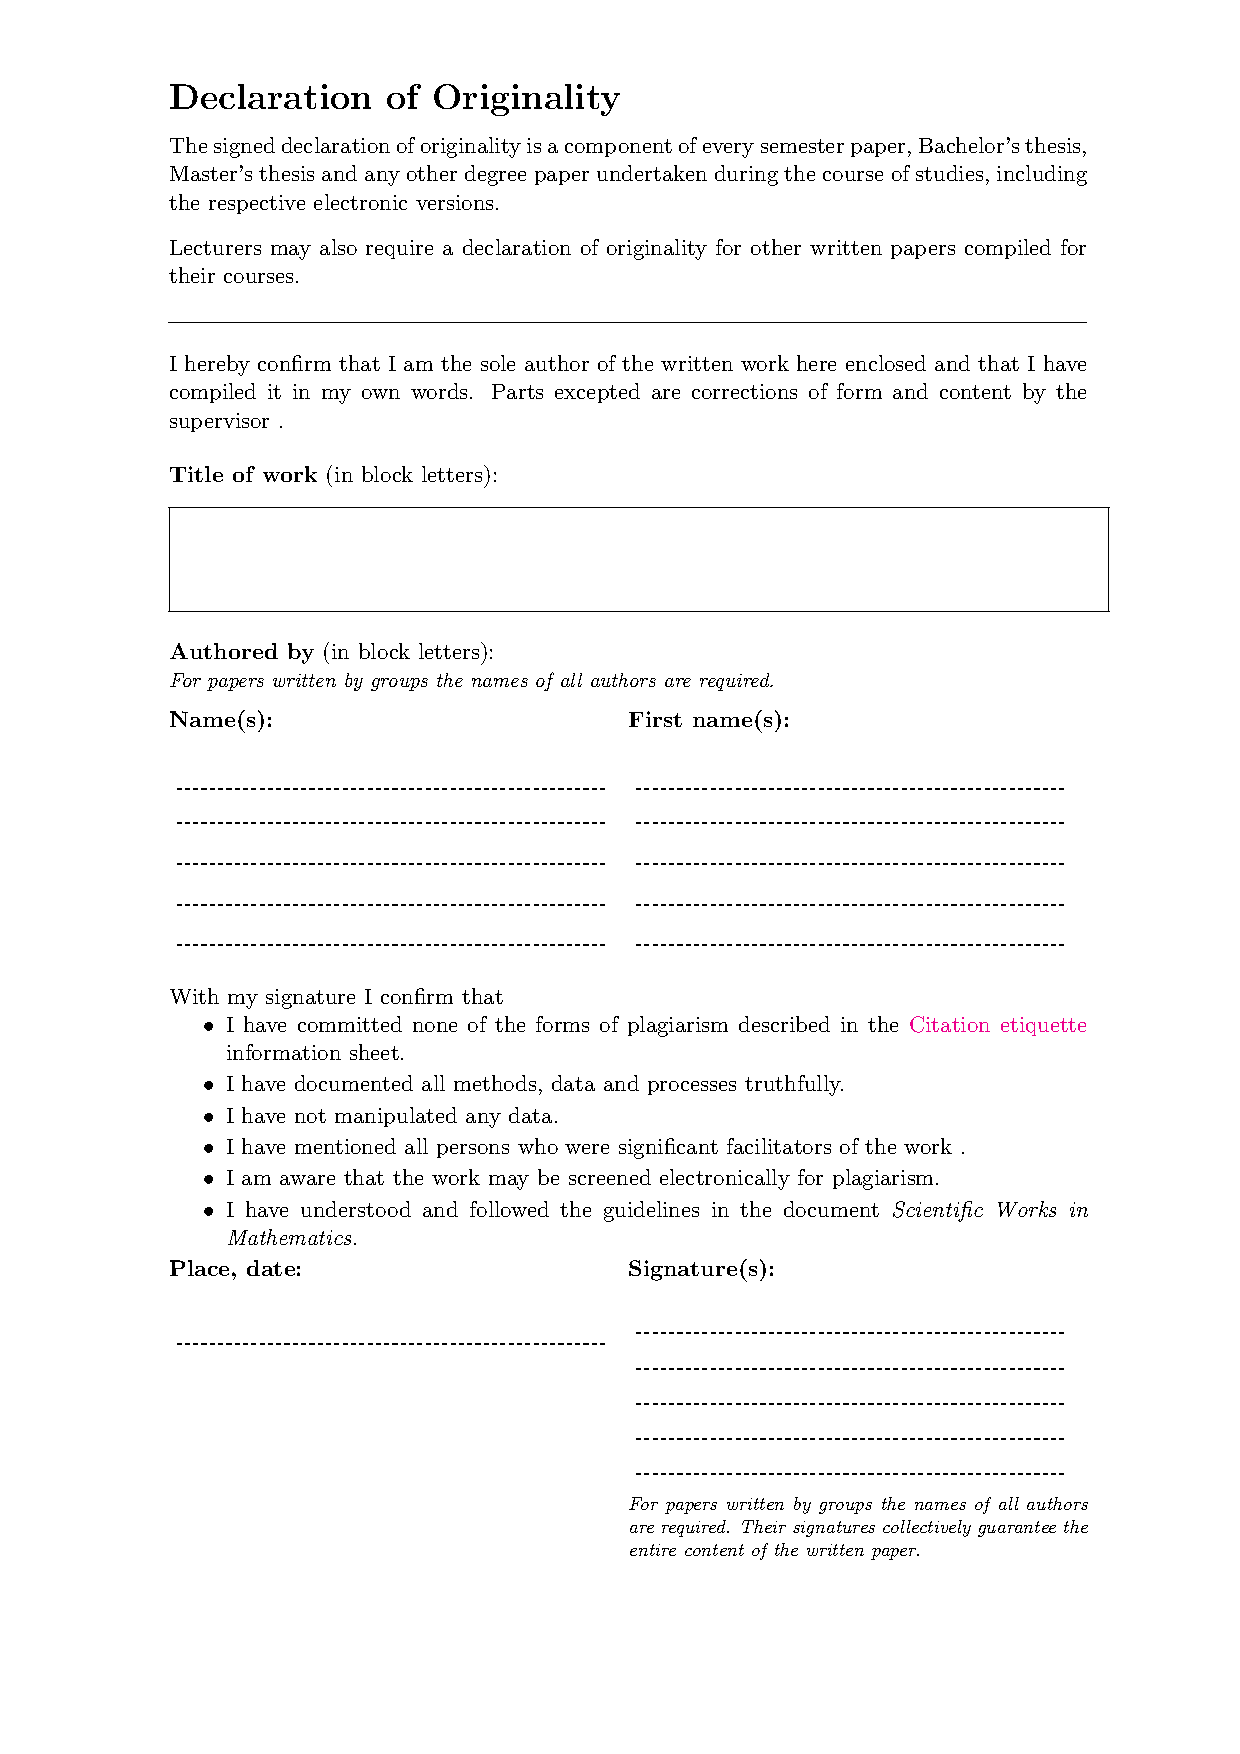
\includepdf[pages={-}, frame=true,scale=1]{pdf/confirmation-originality.pdf}
\end{document}
